\section{Stehende Schallwellen in Luft}

\begin{aufgabe}{Resonanzfrequenzen mit Cassy}
  Geben Sie die Rohrlänge $L$ und ihre Unsicherheit an. Stellen Sie
  Ihre Daten als $U$-$f$-Diagramm dar: Zeichnen Sie Ihre Messpunkte
  ein und verbinden Sie diese ggfs.~mit Linien. Lesen Sie die
  Resonanzfrequenzen $f_n$ ab. Bestimmen Sie die Messunsicherheit auf
  die $f_n$ (Wiederholungsmessung, ersatzweise Abschätzung der
  Genauigkeit, mit der die Peakpositionen abgelesen werden
  können). Zeigen Sie für jede Resonanzfrequenz einen vergrößerten
  Ausschnitt Ihres Diagramms, in den Sie die gefundene Peakposition
  und ihre Unsicherheit einzeichnen. Tragen Sie die $f_n$ gegen $n$
  auf und führen Sie eine lineare Regression durch. Bestimmen Sie die
  Schallgeschwindigkeit und ihre Unsicherheit.
\end{aufgabe}

First we measured the length of the tube we used in our experiment, we obtained the following results conducting independent experiments:
\vspace{1em}
\begin{table}[H]
  \begin{tabular}{c|cc|l}
    Length & Measurements & & Mean \\ \hline
    L & $41,95$ cm & $42$ cm & $41,975$ cm 
  \end{tabular}
\end{table}
we then calculate the uncertainty in our length measurement by quadratically adding our stadard deviation and the sys. error given by the manufacturer of the tool of measurement (in this case a measuring tape with 0,7 mm uncertainty):
$$
\sigma _{L}  =  \sqrt{ \sigma^{2} + \sigma _{sys}^{2} }
$$
$$
\sigma _{L}  =  \sqrt{ 0,35^{2} + (\frac{0,07}{\sqrt{ 3 }})^{2} } \text{ mm} = 0,357 \text{ mm}
$$



we then used scripts to find the first five resonance frequencies, we then sorted our data and noticed that in some of our Measurements we had more than one voltage corresponding to a frequency value so we averaged them and took the peaks of the resulting plot for clarity.
for each of our peaks, we decided that an uncertainty of $2$ Hz is enough to contain the top $10\%-20\%$ of our peak length, and so we took $2$ Hz as conservative frequency uncertainty (highlighted with a red error bar). We then plot our found frequencies and their uncertainties in dedicated plots:




\begin{figure}[H]  
    \centering
    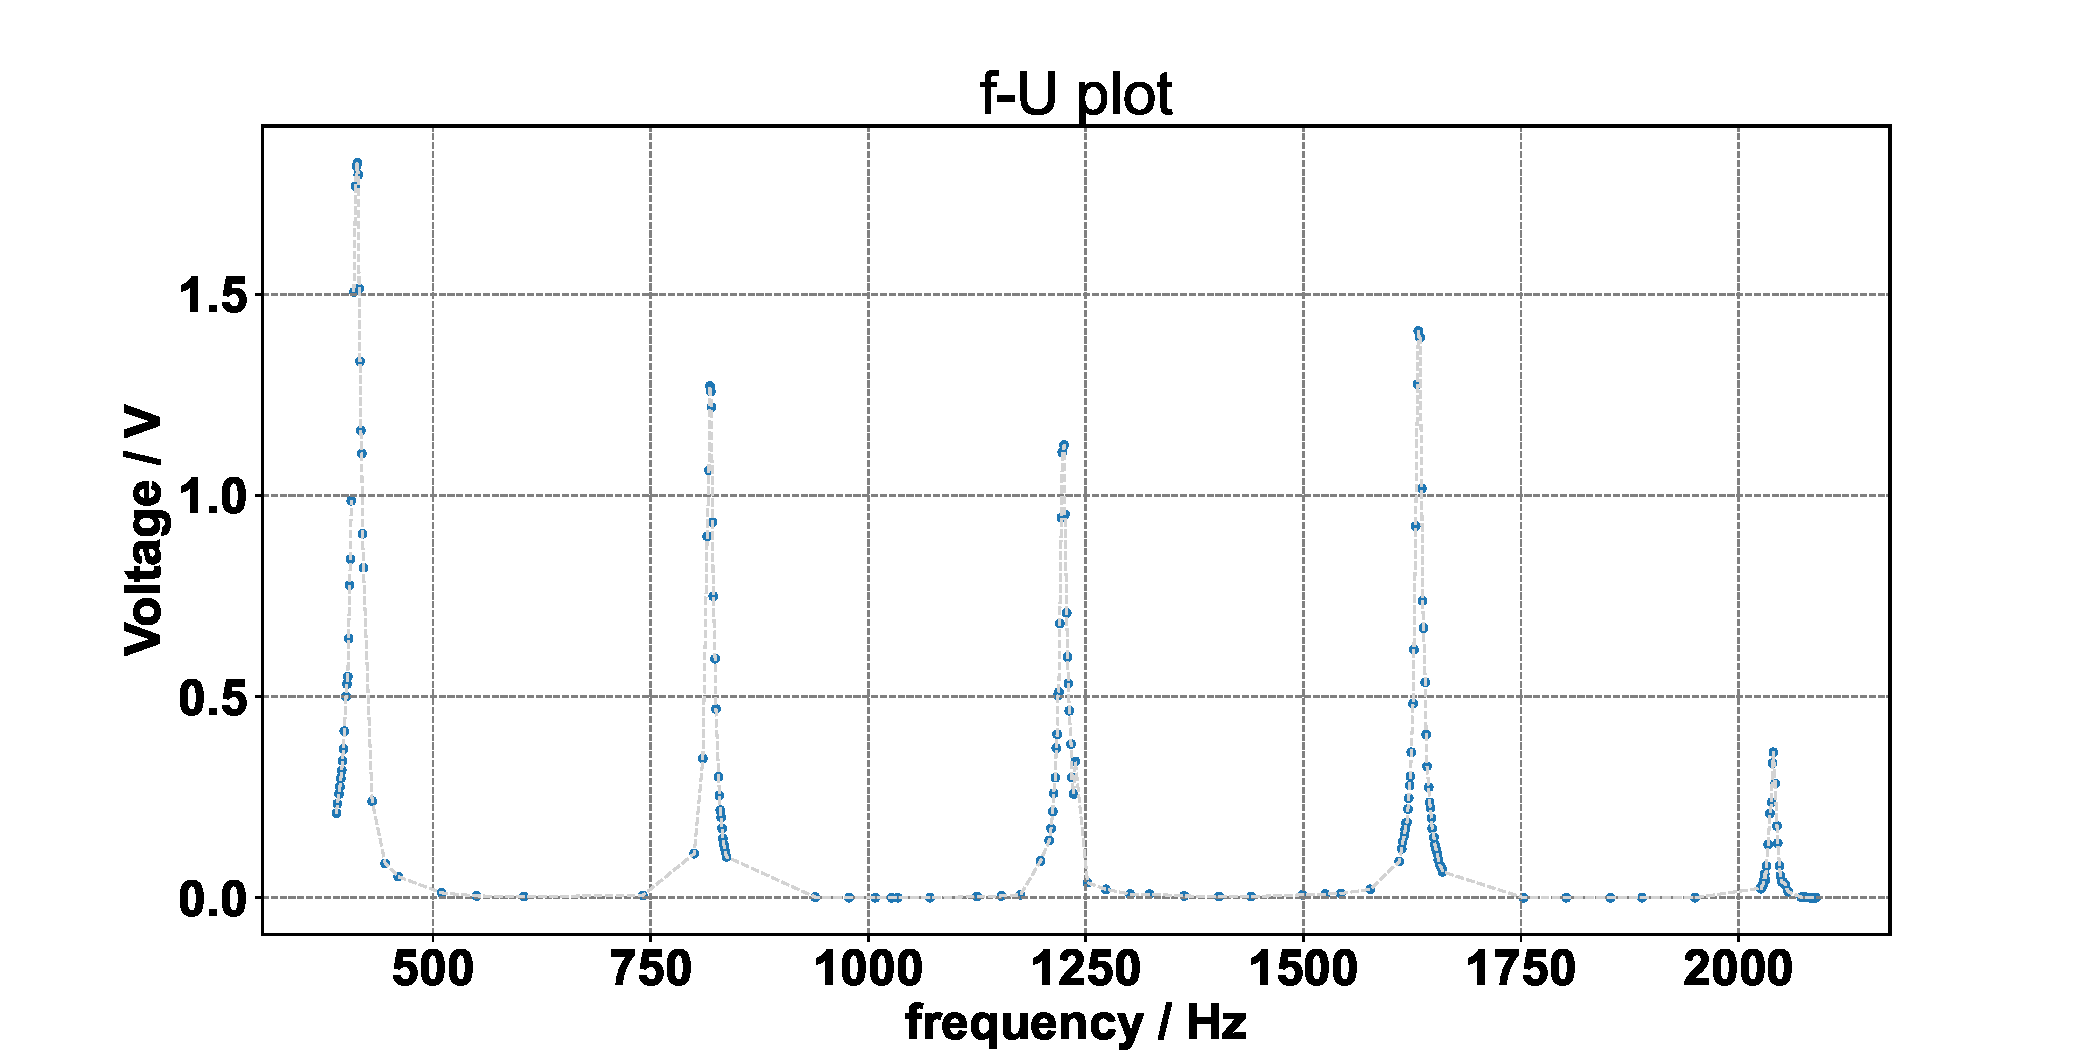
\includegraphics[width=0.8\textwidth]{f_u.pdf}  
    \caption{plot for frequency and voltage}  
    \label{fig:f_1}  
\end{figure}
\begin{figure}[H]  
    \centering
    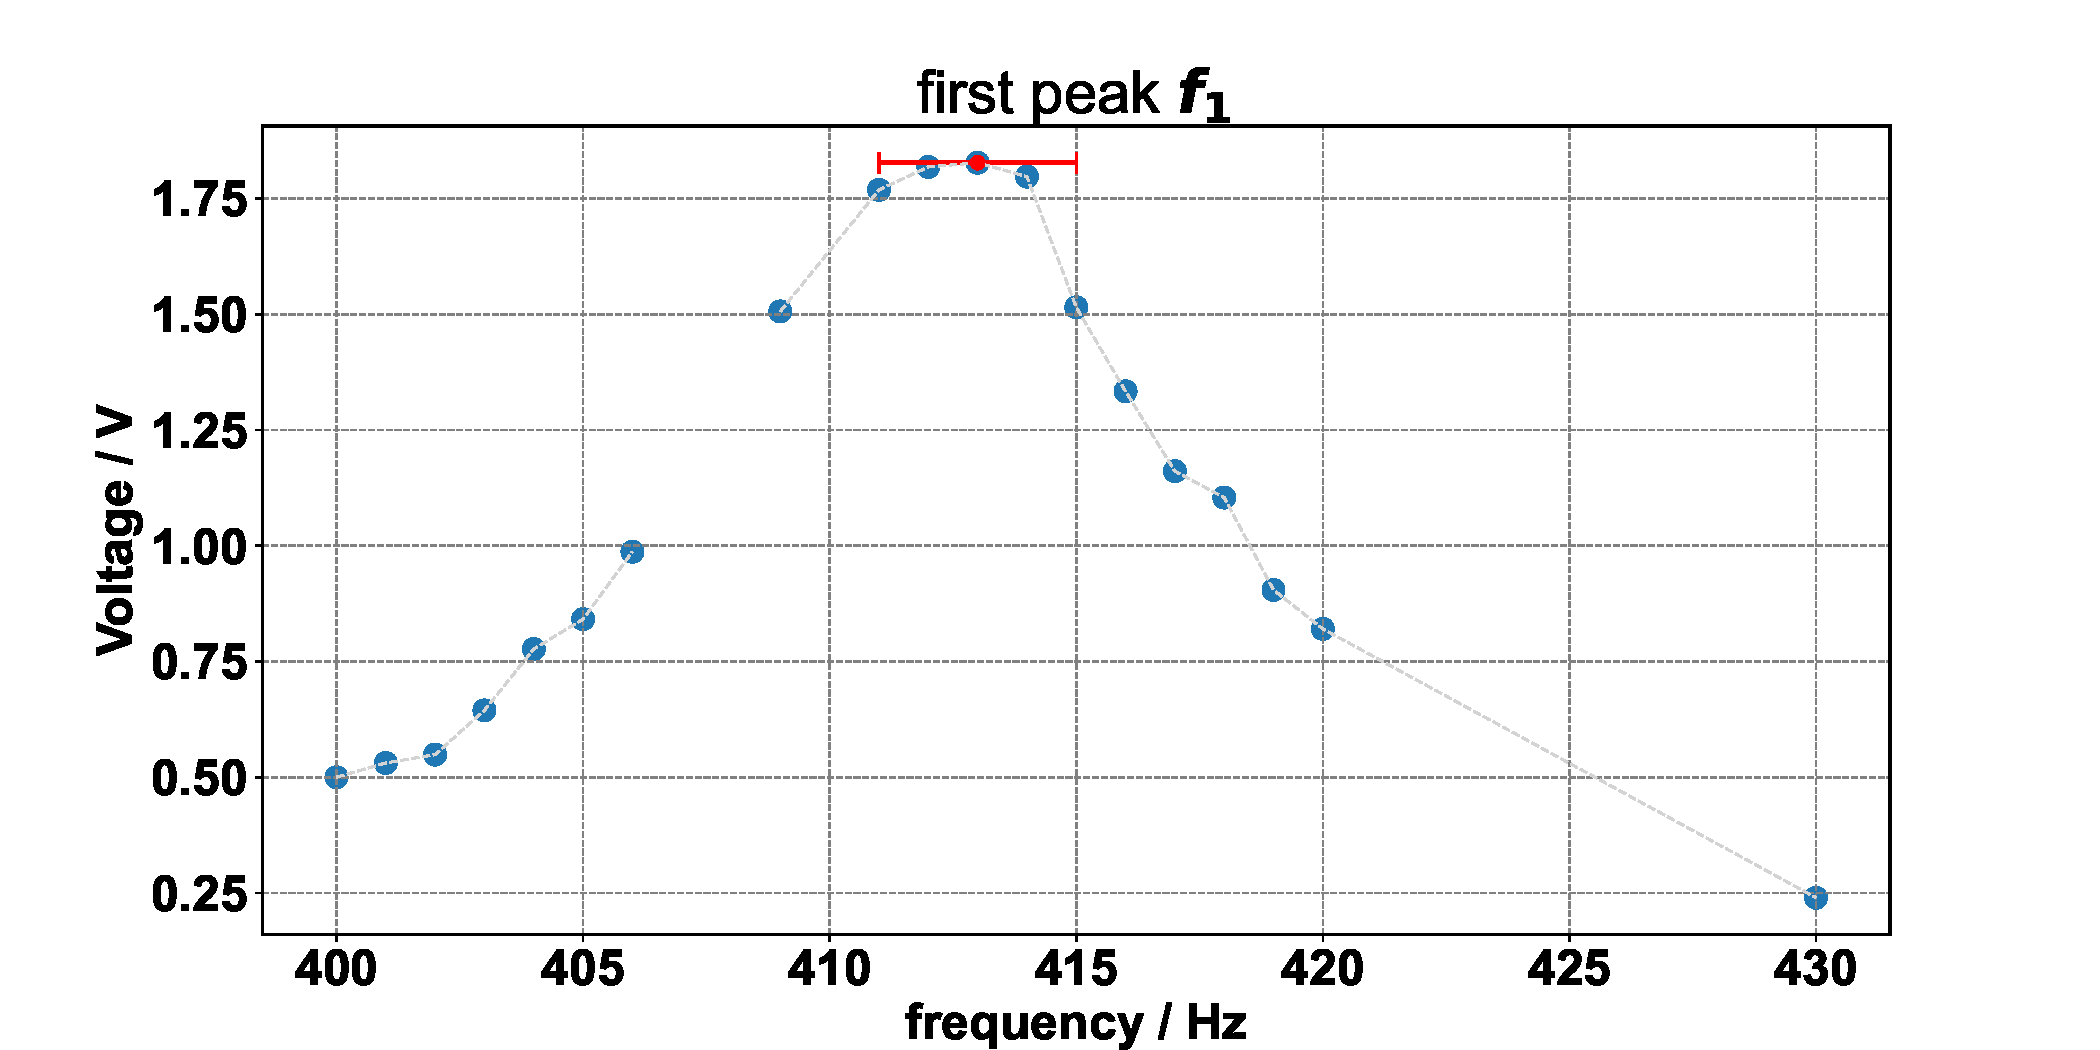
\includegraphics[width=0.8\textwidth]{f_1.pdf}  
    \caption{first frequency}  
    \label{fig:f_1}  
\end{figure}
\begin{figure}[H]  
    \centering
    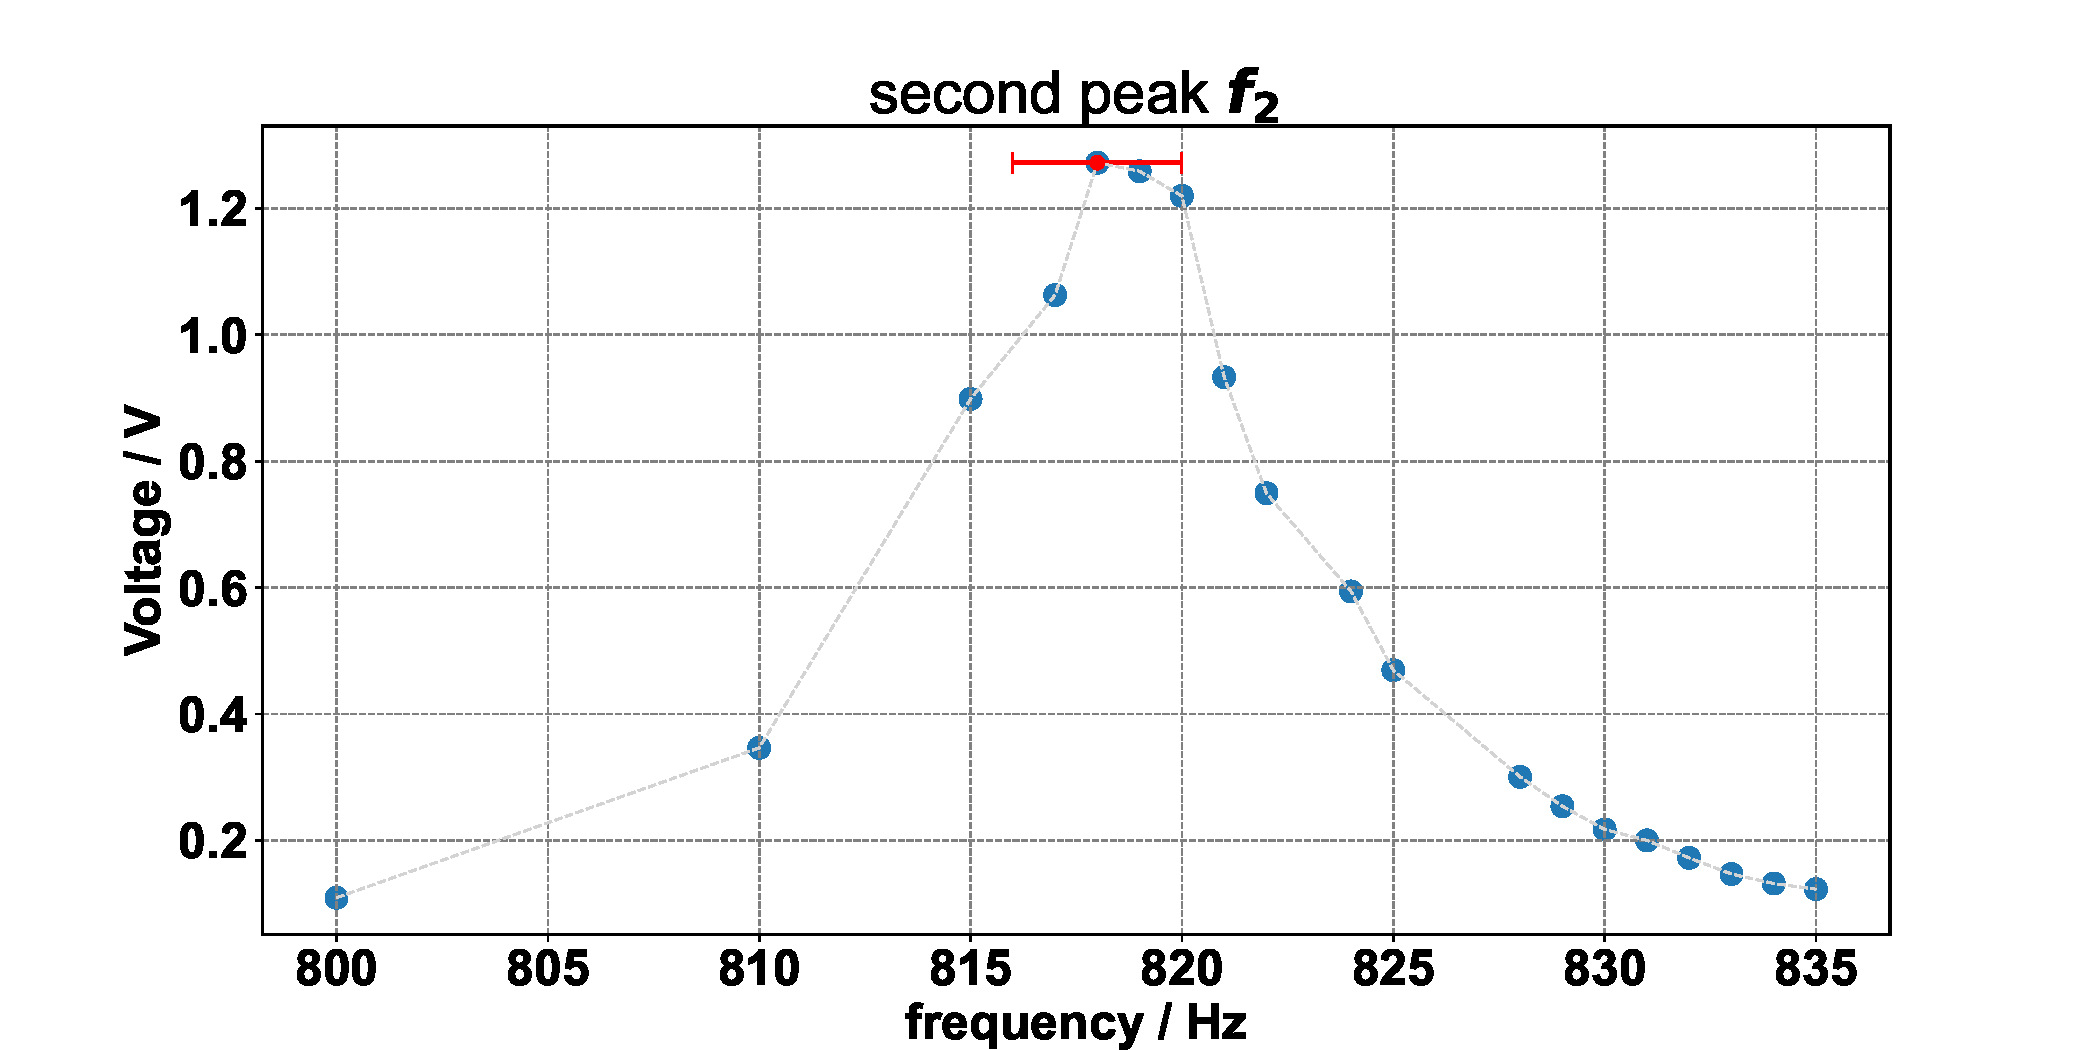
\includegraphics[width=0.8\textwidth]{f_2.pdf}  
    \caption{second frequency}  
    \label{fig:f_2}  
\end{figure}
\begin{figure}[H]  
    \centering
    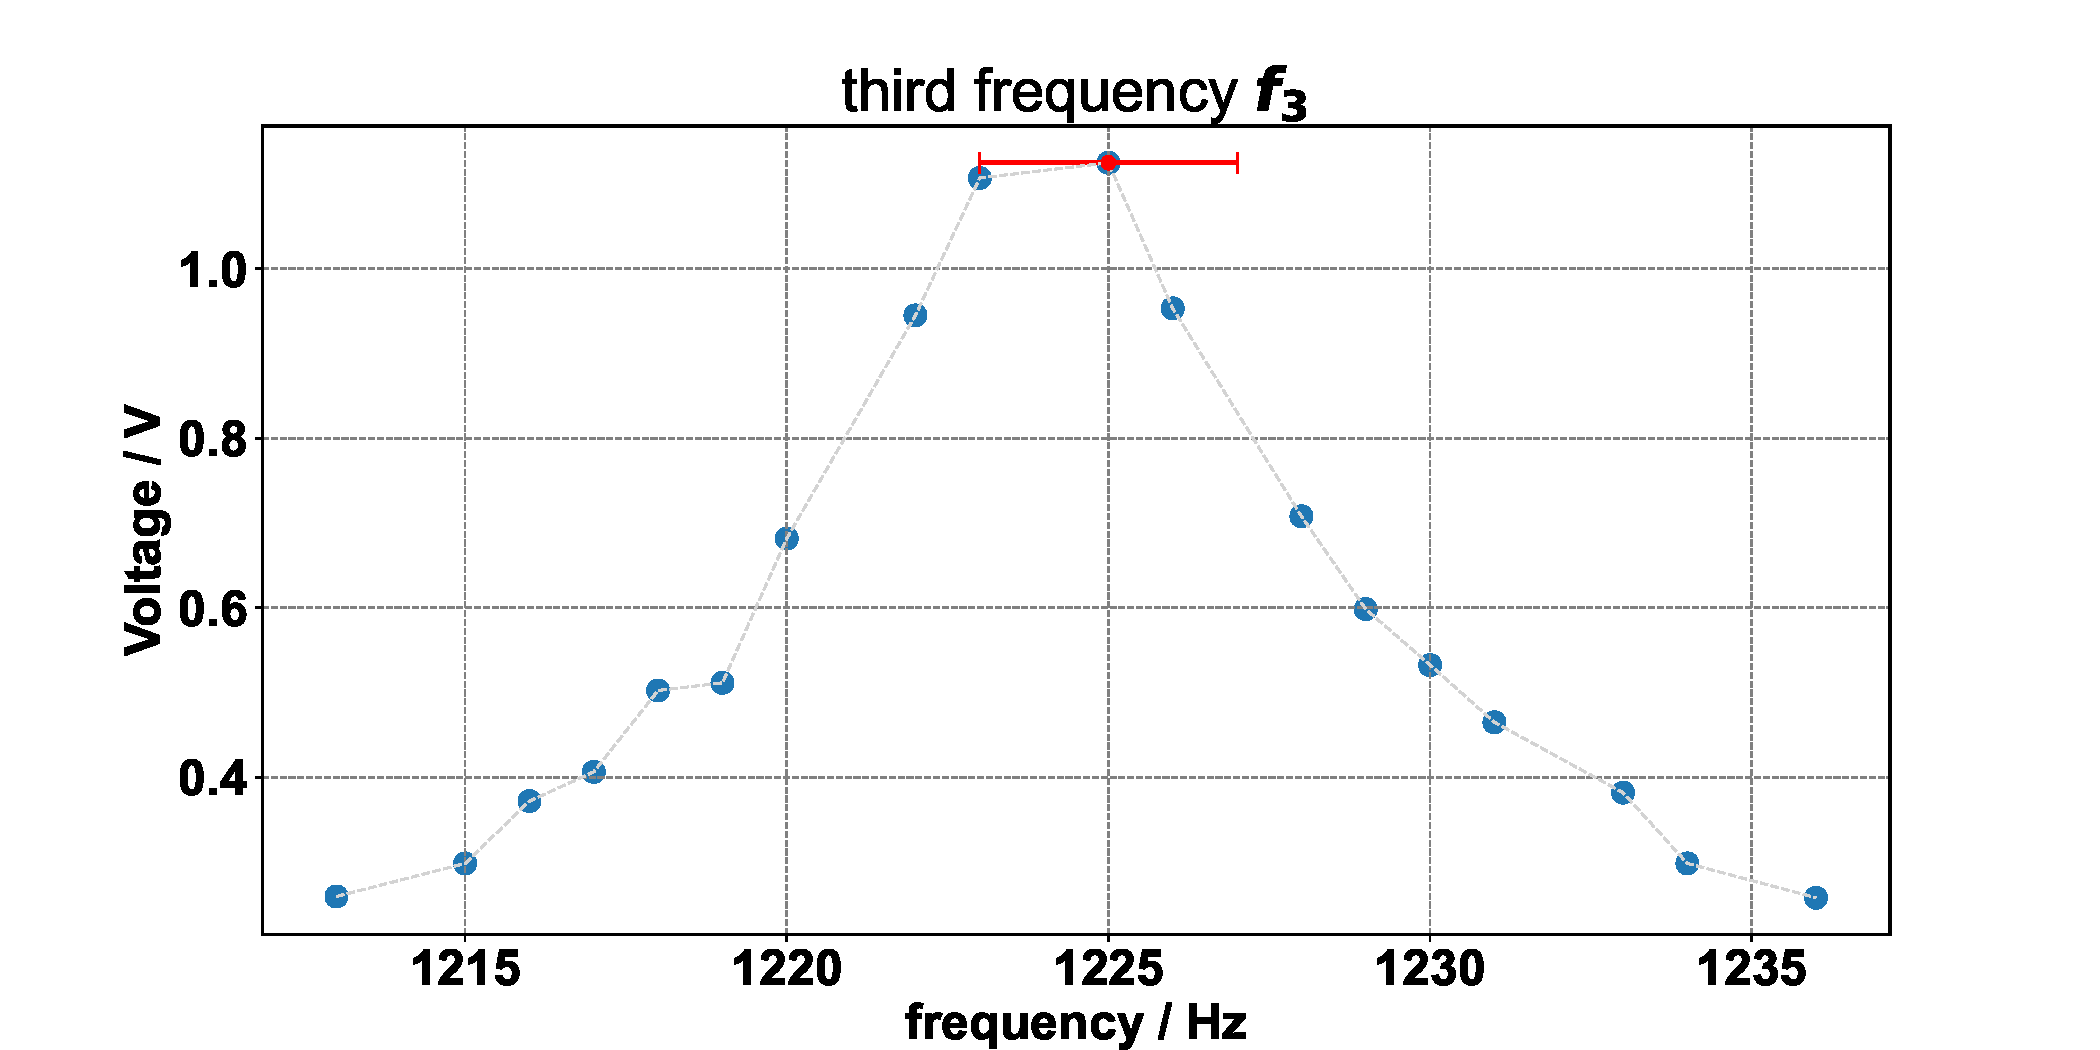
\includegraphics[width=0.8\textwidth]{f_3.pdf}  
    \caption{third frequency}  
    \label{fig:f_3}  
\end{figure}
\begin{figure}[H]  
    \centering
    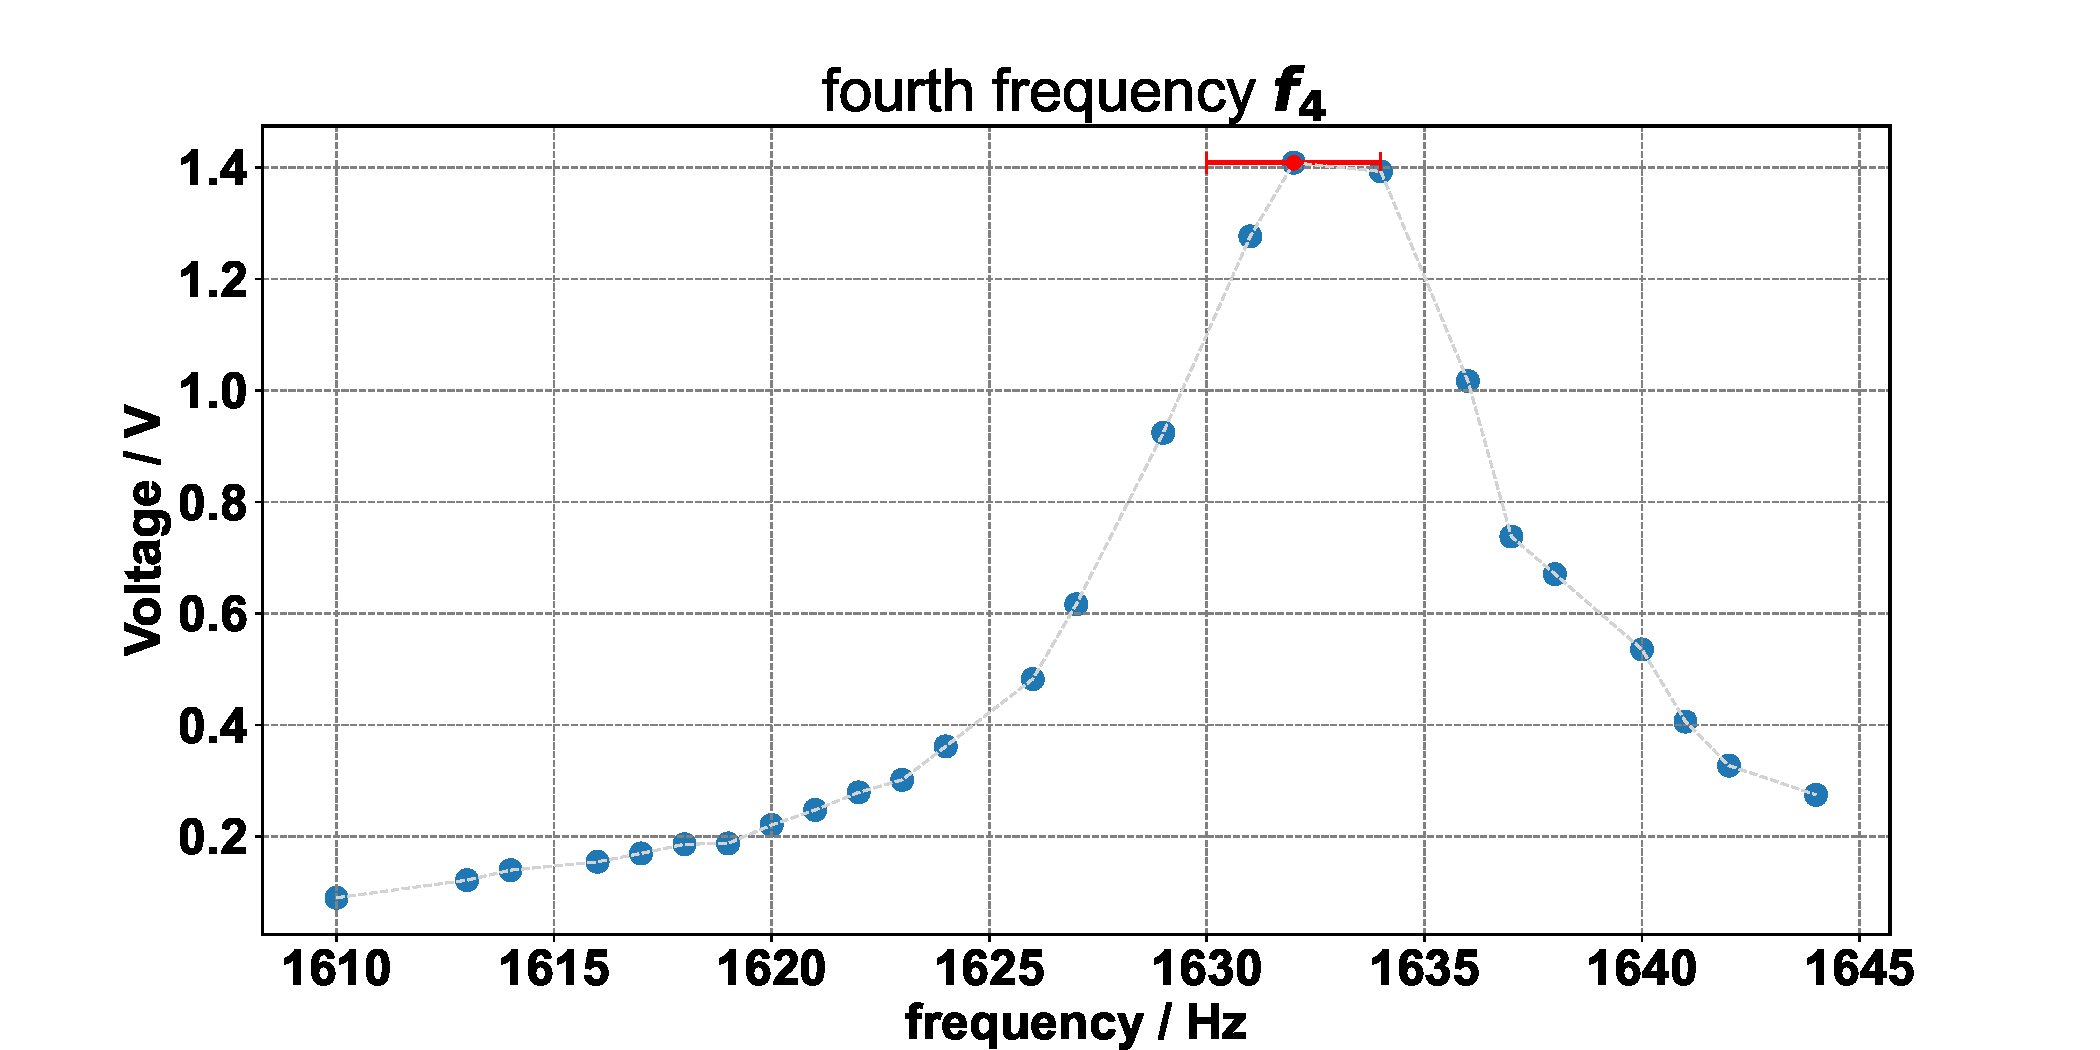
\includegraphics[width=0.8\textwidth]{f_4.pdf}  
    \caption{fourth frequency}  
    \label{fig:f_1}  
\end{figure}
\begin{figure}[H]  
    \centering
    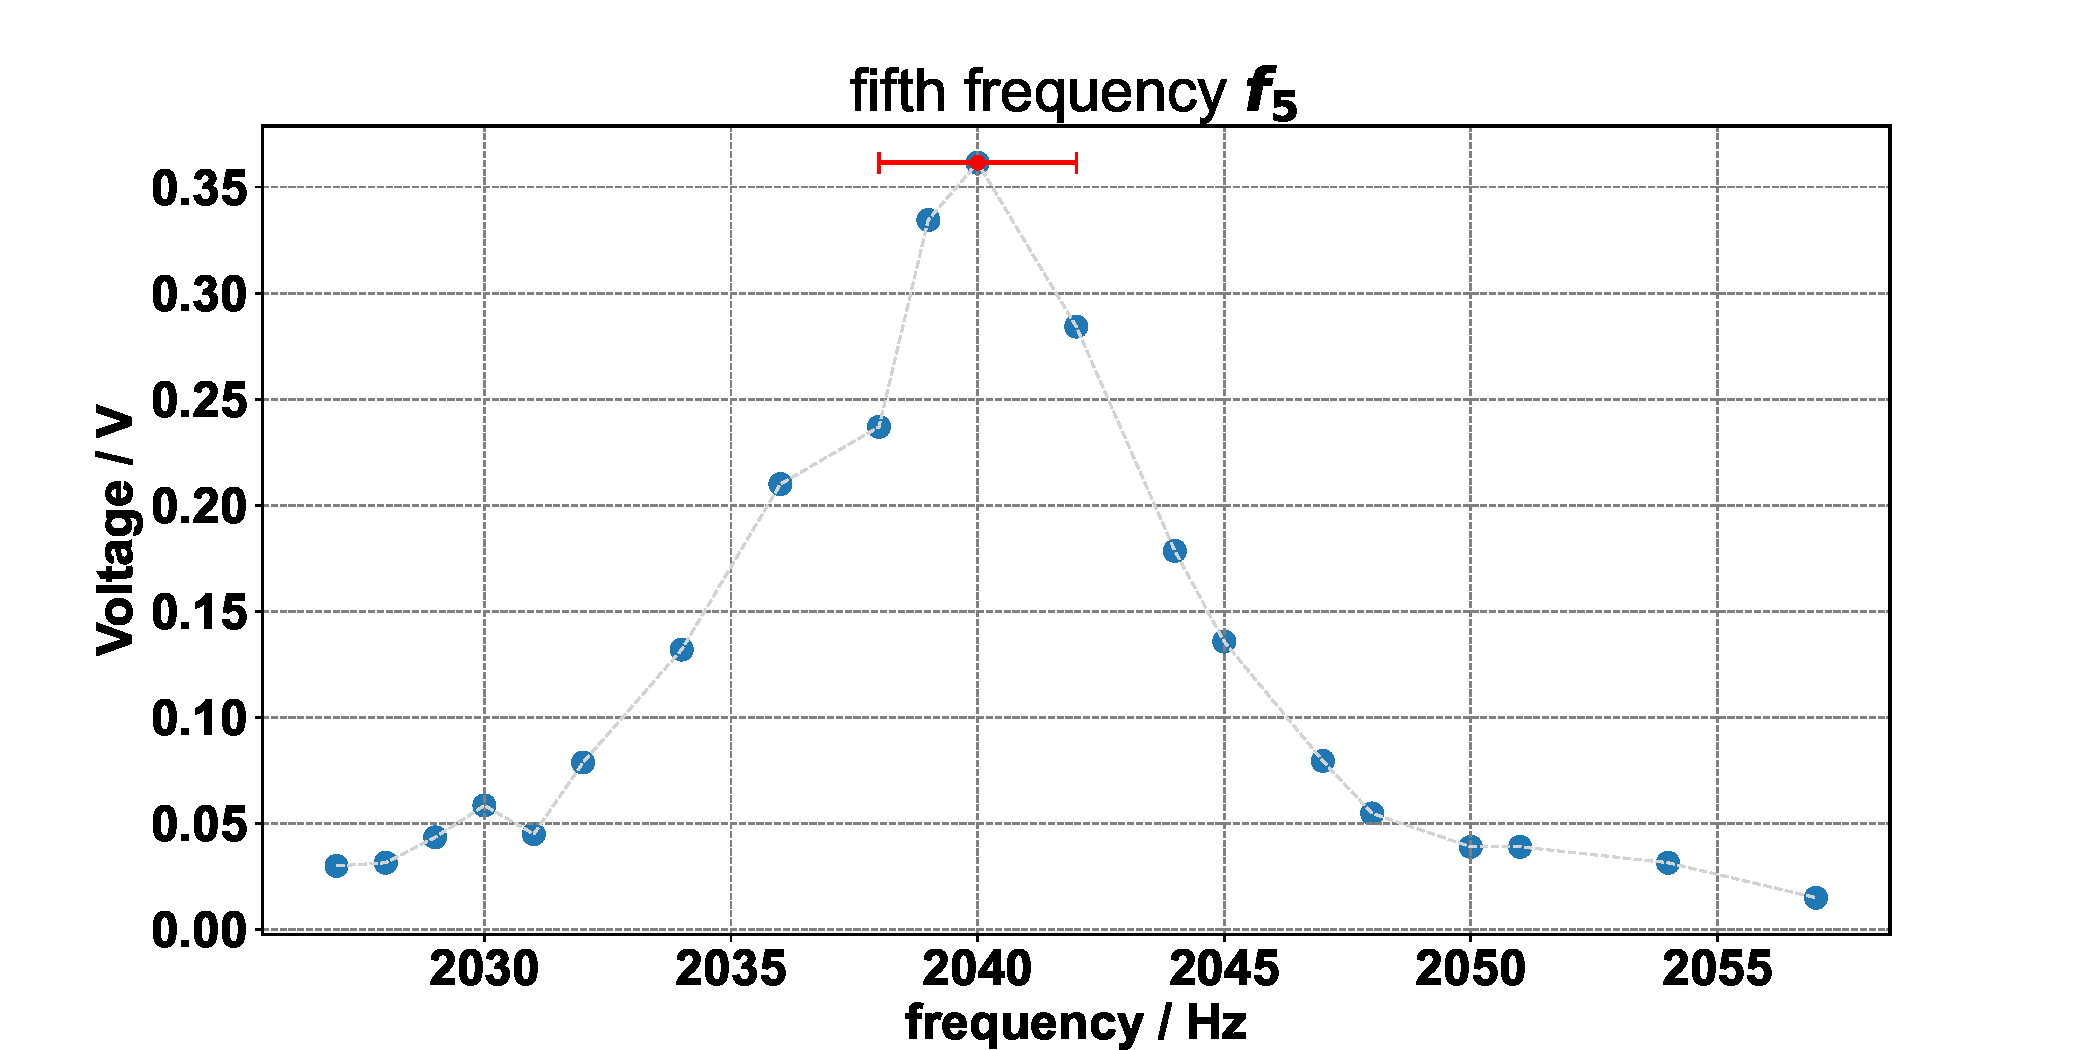
\includegraphics[width=0.8\textwidth]{f_5.pdf}  
    \caption{fifth frequency}  
    \label{fig:f_1}  
\end{figure}

we then give the results of our maximum peaks as follows:
\vspace{1em}
\begin{itemize}
  \item $413$ Hz: first resonance frequency.
  \item $818$ Hz: second resonance frequency.
  \item $1225$ Hz: third resonance frequency.
  \item $1632$ Hz: fourth resonance frequency.
  \item $2040$ Hz: fifth resonance frequency.
\end{itemize}

\vspace{1em}

Then through a linear regression we fit our resonance frequencies to their number, we obtain the following result:

\begin{verbatim}
  R = (406.8+/-0.6) Hz,
  b = (5.2+/-2.1) Hz
  chi2/dof = 0.7 / 3  
  corr = -0.904535
\end{verbatim}
\begin{figure}[H]  
    \centering
    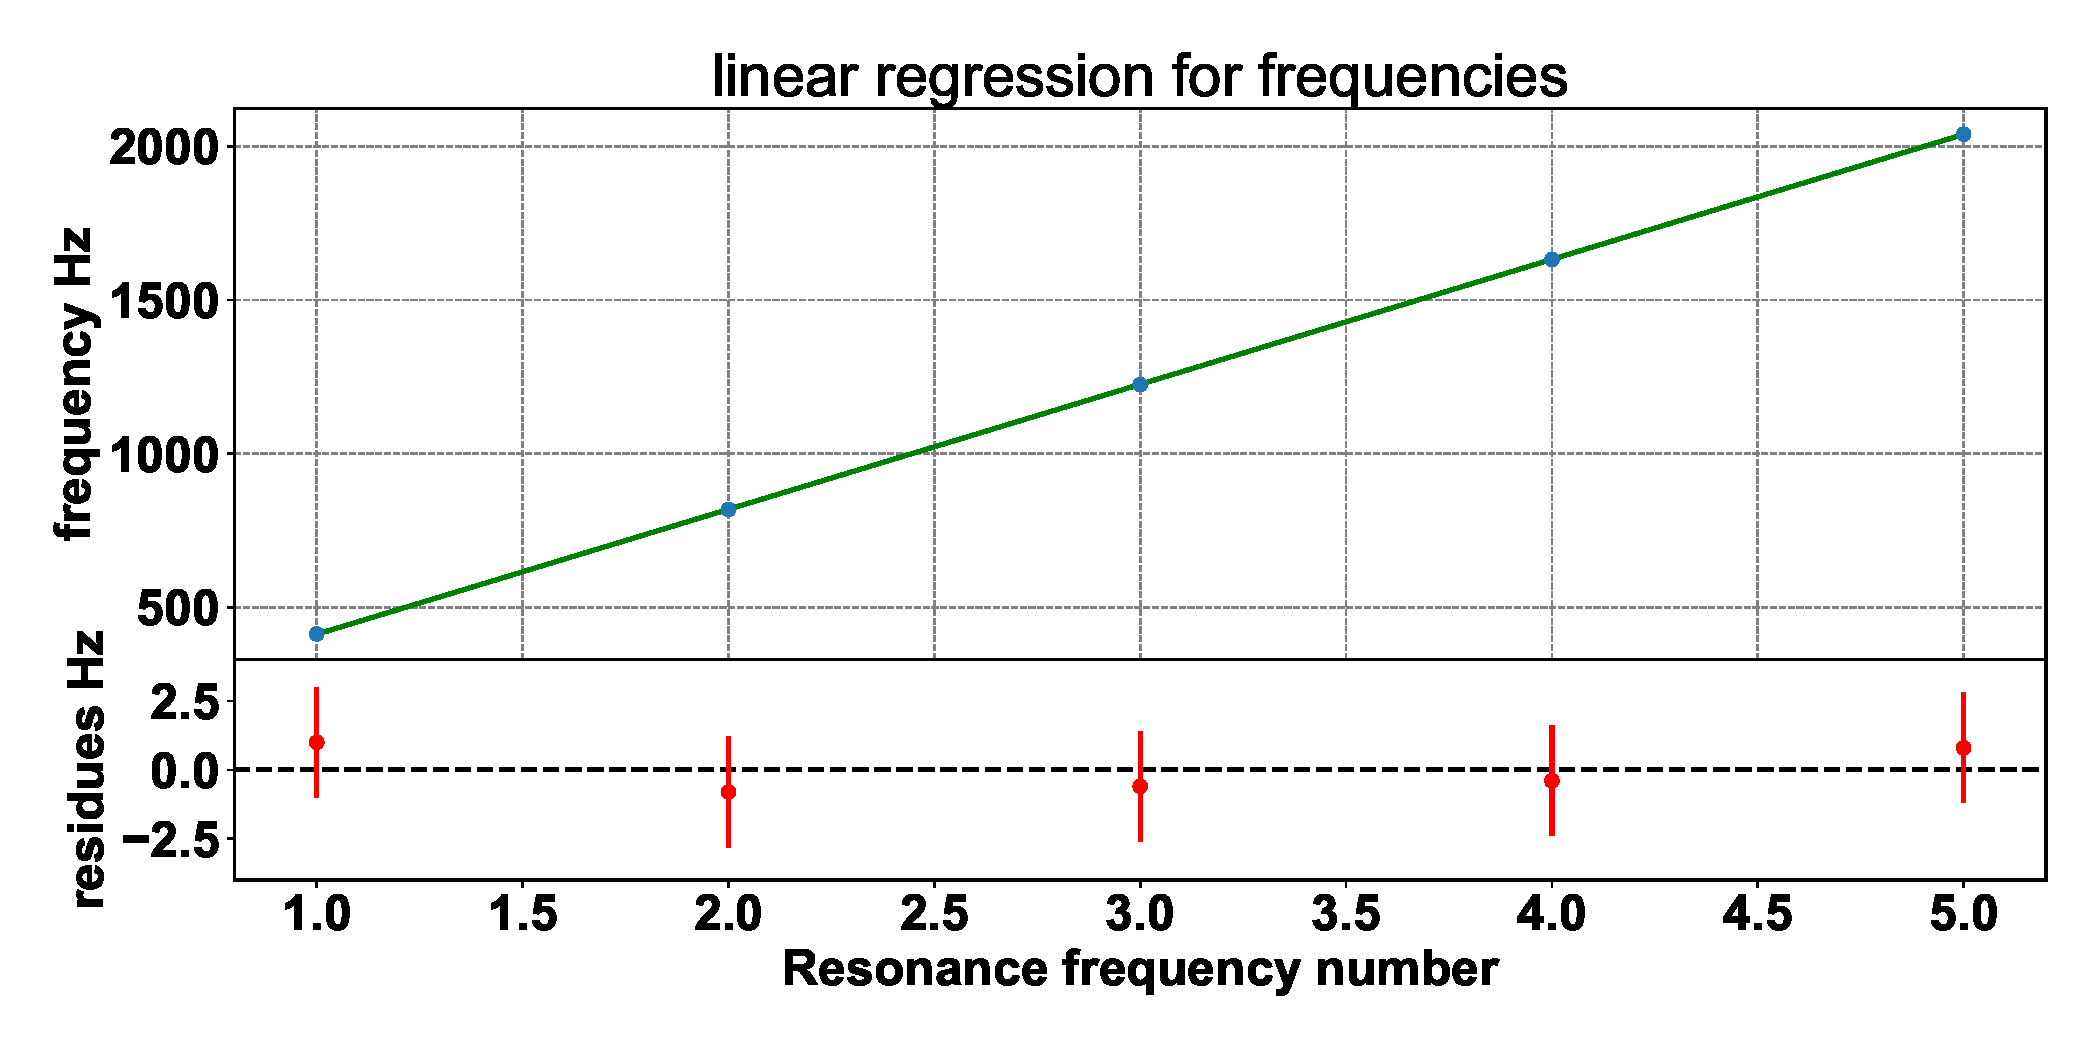
\includegraphics[width=0.8\textwidth]{reg_f_1.pdf}  
    \caption{linear regression fit for frequencies and their numbers}  
    \label{fig:f_1}  
\end{figure}

We then combined our frequencies divided by their number in a variable $f_n /n$ and calculated its uncertainty through weighted average of the resulting division, overall we obtained the following variables and their uncertainties, which leads us to the speed of sound:
$$
v = \frac{f_{n}}{n} \cdot 2 L
$$
\begin{verbatim}
  L: 41,975 +/- 0,357 cm
  f_n / n : 408,2 +/- 0,27 Hz
  v : 342,7 +/- 0,37 m/s
\end{verbatim}














% Bitte belassen Sie die Aufgabentexte in Ihrem Protokoll und beginnen
% Sie hier mit der Lösung der ersten Aufgabe:

% Achten Sie darauf, alle verwendeten Formeln anzugeben und die
% verwendeten Formelzeichen zu definieren.










\begin{aufgabe}{Resonanzfrequenzen mit dem Oszilloskop}
  Tabellieren Sie die gefundenen Resonanzfrequenzen $f_n$. Zur
  Bestimmung der Messunsicherheit auf die $f_n$ führen Sie
  Wiederholungsmessungen durch oder schätzen Sie die Genauigkeit ab,
  mit der Sie die Resonanzfrequenzen mit dem Oszilloskop finden
  können. Bestimmen Sie aus Ihren Messdaten die Schallgeschwindigkeit
  und ihre Unsicherheit. Tragen Sie dazu die $f_n$ gegen $n$ auf und
  führen Sie eine lineare Regression durch.
\end{aufgabe}







\begin{aufgabe}{Vermessung der stehenden Welle}
  Tabellieren Sie die gefundenen Positionen $x_n$ der Druckknoten und
  -bäuche. Geben Sie die jeweils verwendete Resonanzfrequenz $f$ und
  ihre Unsicherheit an. Zur Bestimmung der Messunsicherheit auf die
  $x_n$ führen Sie Wiederholungsmessungen durch oder schätzen Sie die
  Genauigkeit ab, mit der Sie die Druckknoten bzw. -bäuche durch
  Verschiebung des Mikrofons und Beobachtung der Amplitude am
  Oszilloskop einstellen können. Tragen Sie die Positionen $x_n$ gegen
  $n$ auf und führen Sie eine geeignete lineare Regression
  durch. Bestimmen Sie aus Ihren Ergebnissen die Schallgeschwindigkeit
  und ihre Unsicherheit. Berechnen Sie den gewichteten Mittelwert über
  die Ergebnisse aus Ihren Messreihen bei verschiedenen
  Resonanzfrequenzen.
\end{aufgabe}

\begin{aufgabe}{Zusammenfassung und Vergleich}
  Stellen Sie die Ergebnisse aller drei Teilversuche
  nebeneinander. Berechnen Sie ggfs. ein gewichtetes Mittel der
  Schallgeschwindigkeit unter Berücksichtigung der Korrelationen der
  Unsicherheiten. Vergleichen Sie Ihr Ergebnis mit dem Literaturwert
  für die gemessene Raumtemperatur.
\end{aufgabe}
